\documentclass{article}


\usepackage{PRIMEarxiv}

\usepackage[utf8]{inputenc} % allow utf-8 input
\usepackage[T1]{fontenc}    % use 8-bit T1 fonts
\usepackage{hyperref}       % hyperlinks
\usepackage{url}            % simple URL typesetting
\usepackage{booktabs}       % professional-quality tables
\usepackage{amsfonts}       % blackboard math symbols
\usepackage{nicefrac}       % compact symbols for 1/2, etc.
\usepackage{microtype}      % microtypography
\usepackage{amssymb}        % For symbols like checkmark
\usepackage{lipsum}
\usepackage{amsmath}
\usepackage{tikz}
\usetikzlibrary{arrows.meta, positioning, shapes.geometric, fit, calc, decorations.pathreplacing}
\usepackage{fancyhdr}       % header
\usepackage{graphicx}       % graphics
\graphicspath{{media/}}     % organize your images and other figures under media/ folder

%Header
\pagestyle{fancy}
\thispagestyle{empty}
\rhead{ \textit{ }} 

\chead{\underline{\textbf{QuasarV4 Technical Report}}}
\renewcommand{\headrulewidth}{0pt} % Remove the default header rule



  
%% Title
\title{QuasarV4 Technical Report

}

\author{
  Eyad Gomaa \\
  SILX AI \\
  \texttt{eyad.gomaa@silx.ai} \\ % Placeholder email, please update
}

\date{June 9, 2025}


\begin{document}
\maketitle


\begin{abstract}
This is QuasarV4 Technical Report of the 400B/284B AI models with a new transformer architecture, traditional transformer architectures, despite their success, face significant scalability challenges due to the quadratic complexity of their attention mechanisms, limiting context length and incurring substantial computational costs for training state-of-the-art models. This report introduces QuasarV4, a novel transformer architecture developed by SILX AI, designed to overcome these limitations. QuasarV4 achieves linear time and space complexity through a kernel-based linear attention mechanism and incorporates a unique recurrent memory system, enabling effectively infinite context processing. Key architectural components include linear attention with expressive kernel feature maps, an efficient recurrent memory update rule, a hybrid output computation mechanism balancing long-term memory with immediate local context, and Rotary Positional Embeddings (RoPE) for robust relative positional encoding. Furthermore, QuasarV4 integrates several stability techniques to ensure smooth and reliable training. The architecture aims to democratize access to high-performance models by significantly reducing computational demands while maintaining strong reasoning capabilities, paving the way for next-generation AI applications on long-sequence data.
\end{abstract}



\section{Introduction}
Introducing QuasarV4 400B/284B LLMs with a new architecture, the advent of transformer models has revolutionized the field of natural language processing and beyond, demonstrating remarkable capabilities in various tasks. However, the standard self-attention mechanism, a cornerstone of these models, exhibits quadratic complexity with respect to sequence length ($O(N^2)$). This characteristic imposes severe limitations on the practical context window that can be processed and leads to exorbitant computational resource requirements for training and deploying state-of-the-art (SOTA) models on long sequences.

At SILX AI, we have developed the QuasarV4 series of models, a new series of models that use a different, unique transformer architecture designed to directly address these fundamental scalability challenges. QuasarV4 introduces a novel approach that achieves linear time and space complexity ($O(N)$), thereby enabling the processing of effectively infinite context lengths. This is accomplished through a synergistic combination of linear attention mechanisms and an efficient recurrent memory system. Our primary goal with QuasarV4 is to make SOTA-level performance more accessible and computationally feasible, allowing for deeper understanding and modeling of long-form data while maintaining robust reasoning capabilities.

This technical report provides a comprehensive overview of the QuasarV4 architecture. We begin by detailing its core components, including the linear attention mechanism, the recurrent memory system, the hybrid output computation, and the use of Rotary Positional Embeddings. Subsequently, we discuss the various techniques employed to ensure training stability. We also provide an analysis of the model's complexity. Finally, we conclude with a summary of QuasarV4's contributions and its potential impact on future AI research and applications.

\subsection{The Scaling Challenge of Traditional Transformers}
The $O(N^2)$ complexity inherent in the standard self-attention mechanism of transformer models presents a significant bottleneck as sequence lengths ($N$) increase. This quadratic scaling means that doubling the sequence length quadruples the computational load and memory requirements for the attention layers. For instance, processing a sequence of 1000 tokens might be feasible, but scaling to 10,000 tokens would demand 100 times more resources, and 100,000 tokens would require 10,000 times more. This rapid explosion in resource demand has several detrimental consequences:

This rapid explosion in resource demand has several detrimental consequences. Firstly, it practically restricts models to \textbf{Limited Context Windows}, often only a few thousand tokens, as processing longer sequences becomes prohibitively expensive, thereby curtailing their ability to understand long-range dependencies in various sequential data types like text or video. Secondly, it leads to \textbf{High Training Costs}, necessitating massive GPU clusters and extended training periods for large transformers on extensive datasets with long sequences, which in turn makes SOTA research and development accessible primarily to well-resourced organizations. Furthermore, the $O(N^2)$ cost presents significant \textbf{Deployment Challenges}; even during inference, models handling long inputs can be slow and expensive, hindering their real-world application where responsiveness and efficiency are paramount. Lastly, the \textbf{Environmental Impact} is considerable, with the enormous energy consumption associated with training and running these quadratically scaling models raising significant ecological concerns.

This scaling behavior is a primary motivator for developing alternative architectures like QuasarV4, which aim to break free from quadratic constraints and enable efficient processing of much longer sequences.



\section{QuasarV4 Architecture}
The QuasarV4 architecture is built upon several key innovations designed to achieve linear complexity, handle long-range dependencies effectively, and ensure stable training. These components work in concert to provide a powerful and scalable alternative to traditional transformer models.

\subsection{Linear Attention with Kernel Feature Maps}
\label{sec:linear_attention}
The quadratic complexity of standard self-attention, $\text{Attention}(Q, K, V) = \text{softmax}(\frac{QK^T}{\sqrt{d_k}})V$, is a major bottleneck for long sequences. QuasarV4 replaces this with a linear attention mechanism based on kernel feature maps.

The core idea is to approximate the softmax attention using feature maps $\phi(\cdot)$ applied to queries ($Q$) and keys ($K$). The attention computation can be expressed as:
\begin{equation}
\text{Attention}(Q, K, V) \approx \phi(Q) (\phi(K)^T V)
\label{eq:linear_attention_kernel}
\end{equation}
In standard attention, the term $QK^T$ results in an $N \times N$ matrix, where $N$ is the sequence length. By reordering the matrix multiplications as shown in Equation \ref{eq:linear_attention_kernel}, we first compute $\phi(K)^T V$, which is a $d_k \times d_v$ matrix (assuming $\phi$ maps to $d_k$ dimensions). Then, multiplying by $\phi(Q)$ (an $N \times d_k$ matrix) results in an $N \times d_v$ matrix. This reordering avoids the explicit computation of the $N \times N$ attention matrix, reducing the complexity to linear in $N$.

The choice of the feature map $\phi(\cdot)$ is crucial. Desirable properties include:

\begin{itemize}
    \item \textbf{Positivity}: To ensure that the resulting attention scores are non-negative, akin to softmax outputs.
    \item \textbf{Smoothness}: To maintain stable gradients and learning dynamics.
    \item \textbf{Expressiveness}: To capture complex relationships between queries and keys effectively.
\end{itemize}

The path to selecting an optimal feature map $\phi(\cdot)$ for QuasarV4 involved iterative experimentation and analysis. Initial explorations at SILX AI considered several common kernelization approaches, including simpler polynomial kernels and variations of ELU-based feature maps, due to their straightforward implementation. However, these early attempts presented challenges. Some simpler kernels, while computationally lean, lacked the necessary \textbf{Expressiveness}, leading to a noticeable degradation in performance compared to standard softmax attention, particularly on tasks requiring nuanced understanding of token relationships. Achieving consistent \textbf{Positivity} without resorting to ad-hoc clamping or complex transformations that could compromise linearity or introduce bias was another hurdle. Furthermore, training stability was a concern, as certain feature map formulations were prone to numerical issues or gradient instabilities, especially in deeper networks or with longer sequences.

\begin{table*}[t]
    \centering
    \caption{Comparison of Attention Mechanisms. QuasarV4 combines the O(1) decoding of linear attention with an expressive recurrent memory, maintaining linear training complexity while being data-dependent for enhanced modeling.}
    \label{tab:arch_comparison}
    \resizebox{\textwidth}{!}{%
    \begin{tabular}{lcccc}
    \toprule
    \textbf{Model} & \textbf{Attention Matrix (A)} & \textbf{Mechanism} & \textbf{Training Time} & \textbf{Decoding Time \& Space} \\
    \midrule
    Standard Attention & $\sigma(\mathbf{Q}\mathbf{K}^\top)$ & Mask & $O(T^2)$ & $O(T)$ \\
    Linear Attention & $\mathbf{Q}\mathbf{K}^\top$ & Mask & $O(T)$ & $O(1)$ \\
    \midrule
    \textbf{QuasarV4 (Ours)} & $\phi(\mathbf{Q})\phi(\mathbf{K})^\top$ & Recurrent Memory  & $O(T)$ & $O(1)$ \\
    \bottomrule
    \end{tabular}% 
    }
    \end{table*}

Through rigorous empirical evaluation and theoretical investigation, we identified that more sophisticated, learnable feature maps, or those derived from specific mathematical functions designed to better approximate the softmax behavior, offered a more promising direction. The focus shifted towards developing or adapting kernels that could dynamically adjust their expressiveness while inherently satisfying positivity and maintaining a degree of unbiasedness. This led to the adoption of the current kernel feature maps in QuasarV4, which are specifically engineered to provide a strong balance between computational efficiency, modeling power, and training robustness, thereby effectively addressing the limitations encountered with earlier, simpler approaches.

Examples of such feature maps include Exponential Linear Units (ELUs) followed by an offset (e.g., $\phi(x) = \text{elu}(x) + 1$) or other positivity-ensuring functions. This linear attention mechanism allows QuasarV4 to process significantly longer contexts with manageable computational and memory footprints.

\begin{figure}[htbp]
    \centering
    \resizebox{0.5\textwidth}{!}{%
    \definecolor{deepseek_yellow}{HTML}{FFF2CC}
    \definecolor{deepseek_green}{HTML}{C5E0B4}
    \definecolor{deepseek_cyan}{HTML}{DEEBF7}
    \begin{tikzpicture}[
        node distance=0.6cm and 0.8cm, % Vertical and Horizontal distances
        auto,
        >=Stealth,
        main_block/.style={rectangle, draw, fill=deepseek_yellow, rounded corners,
                           text width=4cm, text centered, minimum height=1cm, font=\small},
        op_block/.style={rectangle, draw, fill=deepseek_cyan, rounded corners,
                         text width=2.2cm, text centered, minimum height=0.7cm, font=\scriptsize},
        small_op_block/.style={rectangle, draw, fill=deepseek_green, rounded corners,
                               text width=1.8cm, text centered, minimum height=0.6cm, font=\scriptsize},
        connector_block/.style={rectangle, draw, fill=gray!20, rounded corners,
                                text width=3.5cm, text centered, minimum height=0.8cm, font=\small},
        tensor_label/.style={font=\tiny, text=black},
        path_line/.style={draw, -Stealth},
        head_box/.style={draw, dashed, rounded corners, inner sep=0.4cm} 
    ]

    % Nodes
    \node[main_block] (input_x) {Input $X_t$};
    \node[main_block, right=0.8cm of input_x] (proj_qkv) {Project to $Q, K, V$ \\ ($W_Q, W_K, W_V$)};
    \path[path_line] (input_x) -- (proj_qkv);

    \node[connector_block, text width=2.5cm, fill=gray!10, 
          at={($(input_x.south)!0.5!(proj_qkv.south) - (0,0.9cm)$)}] (split_heads) {Split $N_h$ Heads};
    \draw[path_line, thick] ($(input_x.south)!0.5!(proj_qkv.south)$) to[out=-90, in=90, looseness=1.7] node[tensor_label, right, pos=0.5] {$Q,K,V$} (split_heads);

    % New label node for Single Head Processing
    \node[text width=4cm, text centered, font=\small, below=0.6cm of split_heads] (head_process_label) {Single Head Processing (Head $i$ of $N_h$)};
    \path[path_line, thick] (split_heads.south) -- (head_process_label.north); % Arrow to the new label

    % Q_i, K_i, V_i nodes positioned below the new label
    \node[op_block, below=0.4cm of head_process_label, xshift=-2.8cm] (q_i_node) {$Q_i$};
    \node[op_block, below=0.4cm of head_process_label, xshift=0cm]    (k_i_node) {$K_i$};
    \node[op_block, below=0.4cm of head_process_label, xshift=2.8cm]  (v_i_node) {$V_i$};

    % Arrows from the new label to Q_i, K_i, V_i
    \draw[path_line] (head_process_label.south) to[out=-150, in=150, looseness=1.7] (q_i_node.north);
    \draw[path_line] (head_process_label.south) to[out=-90, in=90, looseness=1.7] (k_i_node.north);
    \draw[path_line] (head_process_label.south) to[out=-30, in=30, looseness=1.7] (v_i_node.north);

    \node[small_op_block, below=of q_i_node] (rope_q) {Apply RoPE};
    \node[small_op_block, below=of k_i_node] (rope_k) {Apply RoPE};
    \path[path_line] (q_i_node) -- (rope_q);
    \path[path_line] (k_i_node) -- (rope_k);

    \node[small_op_block, below=of rope_q] (phi_q) {Apply $\phi(\cdot)$};
    \node[small_op_block, below=of rope_k] (phi_k) {Apply $\phi(\cdot)$};
    \path[path_line] (rope_q) -- node[tensor_label, left, pos=0.5] {$Q'_i$} (phi_q);
    \path[path_line] (rope_k) -- node[tensor_label, right, pos=0.5] {$K'_i$} (phi_k);

    % Kernelized Linear Attention Breakdown
    \node[op_block, align=center, below=0.8cm of phi_k] (kv_context) {Compute Key-Value Context};
    \draw[path_line] (phi_k.south) to[out=-90, in=90, looseness=1.0] node[tensor_label, pos=0.3, right=-2pt] {$\phi(K'_i)$} (kv_context.north); % Straight down from phi_k
    \draw[path_line] (v_i_node.south) to[out=-90, in=0, looseness=1.2] node[tensor_label, pos=0.3, above right=-2pt] {$V_i$} (kv_context.east); % From V_i (right) into east side of kv_context

    \node[op_block, align=center, below=0.8cm of kv_context] (attend_q) {Attend with Query};
    \draw[path_line] (kv_context.south) to[out=-90, in=90, looseness=1.0] (attend_q.north); % Straight down from kv_context
    \draw[path_line] (phi_q.south) to[out=-90, in=180, looseness=1.2] node[tensor_label, pos=0.3, above left=-2pt] {$\phi(Q'_i)$} (attend_q.west); % From phi_q (left) into west side of attend_q
    
    \node[head_box, fit=(q_i_node) (k_i_node) (v_i_node) (rope_q) (rope_k) (phi_q) (phi_k) (kv_context) (attend_q)] (head_proc_box) {};

    \node[connector_block, below=0.8cm of head_proc_box.south] (concat) {Concatenate Head Outputs};
    \path[path_line] (attend_q.south) -- node[tensor_label, right, pos=0.5] {$\text{HeadOut}_i$} (concat.north);

    \node[main_block, below=of concat] (proj_o) {Final Linear Projection $W_O$};
    \path[path_line] (concat) -- (proj_o);

    \node[main_block, below=of proj_o] (output_o) {Output $O_t$};
    \path[path_line] (proj_o) -- (output_o);

    \end{tikzpicture}
    }
    \caption{QuasarV4 Multi-Head Linear Attention with RoPE and Kernel Feature Maps $\phi(\cdot)$.}
    \label{fig:quasar_mha_kernel}
\end{figure}


\subsection{Recurrent Memory Mechanism}
\label{sec:recurrent_memory}
To handle arbitrarily long sequences and maintain information over extended contexts, QuasarV4 incorporates a compressed recurrent memory matrix, $M_t$. This matrix serves as a summary of past information, updated at each timestep $t$. The update rule is defined as:
\begin{equation}
M_t = \alpha M_{t-1} + \phi(K_t)^T V_t
\label{eq:memory_update}
\end{equation}
Here, $M_{t-1}$ is the memory state from the previous timestep, $\phi(K_t)^T V_t$ represents the new information from the current key-value pair (processed through the same feature map $\phi$ as in linear attention), and $\alpha$ is a learnable or fixed decay factor.


\begin{figure}[htbp]
   \resizebox{0.9\textwidth}{!}{%
    \centering
    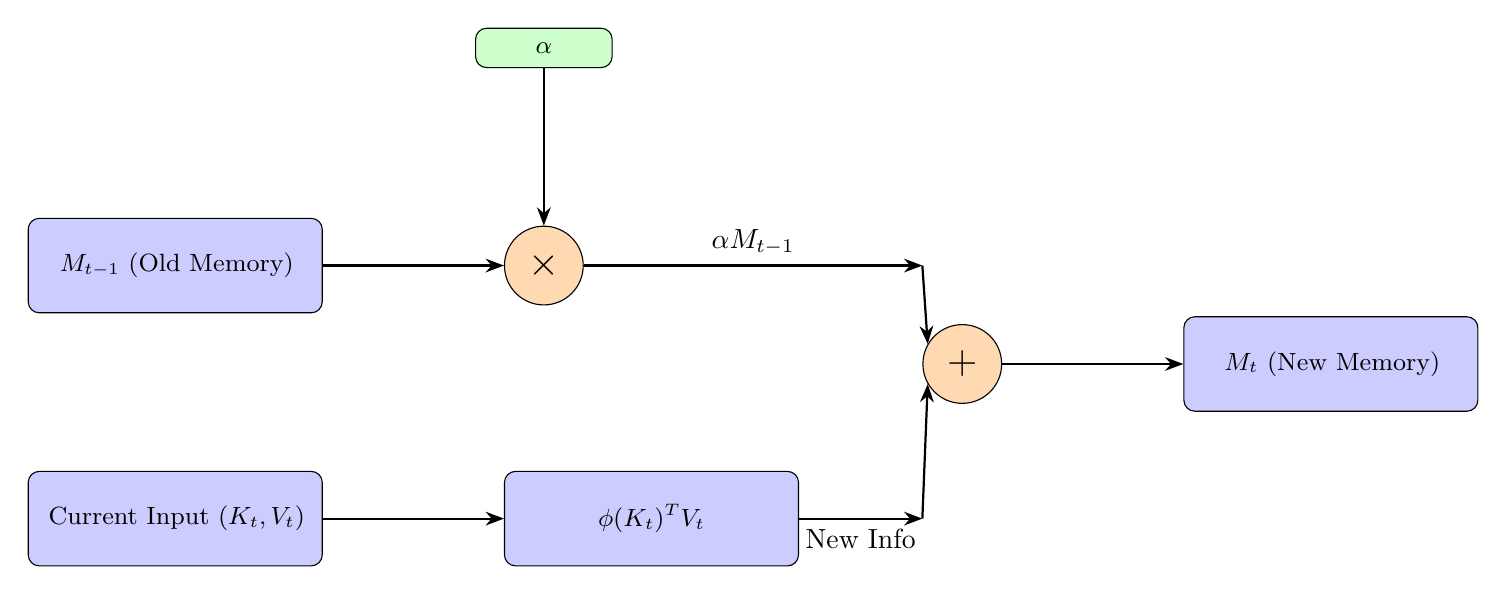
\begin{tikzpicture}[node distance=1.5cm and 2.5cm, auto, >=Stealth,
        block/.style={rectangle, draw, fill=blue!20, text width=3.5cm, text centered, rounded corners, minimum height=1.2cm, font=\small},
        op_block/.style={circle, draw, fill=orange!30, minimum size=1cm, font=\Large},
        label_block/.style={rectangle, draw, fill=green!20, text width=1.5cm, text centered, rounded corners, minimum height=0.5cm, font=\small},
        line/.style={draw, -Stealth, thick}]

        % Nodes
        \node [block] (mt_minus_1) {$M_{t-1}$ (Old Memory)};
        \node [op_block, right=of mt_minus_1, xshift=-0.2cm] (alpha_op) {$\times$};
        \node [label_block, above=of alpha_op, yshift=0.5cm] (alpha_label) {$\alpha$};

        \node [block, below=of mt_minus_1, yshift=-0.5cm] (current_input) {Current Input ($K_t, V_t$)};
        \node [block, right=of current_input, xshift=-0.2cm] (phi_k_v) {$\phi(K_t)^T V_t$};
        
        \node [op_block, right=of alpha_op, xshift=1.8cm, yshift=-1.25cm] (sum_op) {$+$};
        \node [block, right=of sum_op, xshift=-0.2cm] (mt) {$M_t$ (New Memory)};

        % Paths
        \path [line] (current_input.east) -- (phi_k_v.west); % Connect Current Input to its transformation
        \path [line] (mt_minus_1.east) -- (alpha_op.west); % From M_t-1 block to X operator
        \path [line] (alpha_label.south) -- (alpha_op.north); % From alpha label to X operator
        
        % Define coordinates for the end of the horizontal segments stemming from X and phi_k_v
        % These coordinates will be at the same x-level as the sum operator's left side
        \coordinate (end_horizontal_alpha) at (sum_op.west |- alpha_op.east);
        \coordinate (end_horizontal_phi) at (sum_op.west |- phi_k_v.east);

        % Draw the horizontal lines with their labels
        \path [line] (alpha_op.east) -- (end_horizontal_alpha) node[above, midway] {$\alpha M_{t-1}$};
        \path [line] (phi_k_v.east) -- (end_horizontal_phi) node[below, midway] {New Info};
        
        % Draw lines connecting the end of these horizontal segments to the sum operator
        % Using angled anchors (150 degrees for top-left, 210 for bottom-left) for the circular sum operator
        \path [line] (end_horizontal_alpha) -- (sum_op.150); 
        \path [line] (end_horizontal_phi) -- (sum_op.210);   
        
        % Draw the line from the sum operator to the new memory block
        \path [line] (sum_op.east) -- (mt.west);
    \end{tikzpicture}
   }
    \caption{Visualization of the Recurrent Memory Update Mechanism in QuasarV4. The previous memory state $M_{t-1}$ is decayed by $\alpha$, and new information derived from the current key $K_t$ and value $V_t$ (via feature map $\phi$) is added to form the new memory state $M_t$.}
    \label{fig:memory_update_viz}
\end{figure}

The memory matrix $M_t$ is a crucial component, acting as a compressed, fixed-size representation of the entire history seen up to timestep $t$. Its dimensions (e.g., $d_k \times d_v$) are independent of the sequence length $N$, which is key to the model's scalability. The update rule in Equation \ref{eq:memory_update} can be intuitively understood as an exponential moving average. The existing memory $M_{t-1}$ is scaled down by the decay factor $\alpha$, effectively "forgetting" a small portion of older information. Simultaneously, new information, encapsulated by the term $\phi(K_t)^T V_t$, is incorporated. This term represents the outer product of the current transformed key $\phi(K_t)$ and the current value $V_t$. It essentially adds the "knowledge" or "observation" from the current timestep into the memory, associating the current key's features with its corresponding value. Because $M_t$ maintains a constant size, each update step is computationally efficient, contributing to the overall linear time complexity per layer with respect to sequence length.

The decay factor $\alpha$ (typically close to 1, e.g., $0.9 \text{ to } 0.999$) controls the balance between retaining past information and incorporating new data. A value closer to 1 emphasizes long-term retention, while a smaller value allows the memory to adapt more quickly to recent inputs. This mechanism allows QuasarV4 to maintain an effectively infinite-length memory with a fixed-size storage for $M_t$, making it highly scalable for very long sequences.

\subsection{Hybrid Output Computation}
\label{sec:hybrid_output}
QuasarV4 employs a hybrid approach to compute its output at each timestep, combining information from the long-term recurrent memory $M_{t-1}$ with information from the immediate local context (derived from a local attention window or the current input directly). This balance is dynamically controlled by a learnable gating vector $g_t$:
\begin{equation}
O_t = (1 - g_t) \odot \underbrace{\text{LocalAttnOut}_t}_{\text{Immediate Context}} + g_t \odot \underbrace{(\phi(Q_t) M_{t-1})}_{\text{Long-term Memory Context}}
\label{eq:hybrid_output}
\end{equation}
where $\odot$ denotes element-wise multiplication.

\subsection{Pretraining}
\label{sec:pretraining}
The QuasarV4 series of models is pretrained on an extensive dataset of 15 trillion tokens, encompassing diverse sources such as mathematical texts, source code, and other specialized and general-purpose corpora. Pretraining such large-scale architectures can be challenging due to issues such as vanishing or exploding gradients. To ensure a stable and effective learning process, QuasarV4 incorporates several established techniques. These include robust normalization layers (such as LayerNorm or RMSNorm) applied strategically within the architecture to maintain consistent activation scales. For managing long-range dependencies during training with recurrent components, Truncated Backpropagation Through Time (TBPTT) is employed to limit the length of gradient propagation, making the process more computationally tractable and stable. Furthermore, Gradient Clipping is utilized to prevent excessively large gradient updates, which can destabilize training, by capping gradient norms at a predefined threshold. These methods collectively contribute to a smoother and more reliable pretraining phase, enabling QuasarV4 to effectively learn from its vast dataset.

\textbf{DeepSeek-V3 Mixture-of-Experts (MoE) Integration:}
To further enhance scalability and parameter efficiency during its extensive pretraining, the QuasarV4 architecture was augmented with a sparse Mixture-of-Experts (MoE) model. This approach modifies the traditional dense feed-forward networks within the transformer blocks. Instead of activating all parameters in a layer, MoE routes each input token to a small subset of "expert" networks (typically MLPs), enabling significant model scaling without a proportional increase in computational cost per token. QuasarV4 implements a Top-2 routing mechanism, where each token is processed by the two most suitable experts.

The general flow within a QuasarV4 transformer block incorporating MoE is as follows: Input token embeddings pass through the block's attention mechanisms (QuasarV4's linear attention and recurrent memory interactions) and then to the MoE layer, before any residual connections and layer normalization leading to the next block or output head. The MoE layer implementation in QuasarV4 closely follows the architecture used in models like DeepSeek-V3, notably employing its Top-2 routing mechanism. This approach incorporates the necessary components for efficient expert selection, sparse activation of expert networks, and load balancing strategies to ensure stable and effective training with a large number of experts.
This MoE integration is designed to be compatible with QuasarV4's core architectural innovations, such as its linear attention and recurrent memory system, by primarily replacing or augmenting the dense MLP layers within the transformer blocks. This allows QuasarV4 to leverage the benefits of sparse expert models while retaining its unique capabilities for efficient long-context processing.


The hybrid output mechanism is designed to endow QuasarV4 with the ability to flexibly integrate information from different temporal scales. Relying solely on long-term memory might smooth out or miss critical recent details, while depending only on local context would prevent the model from leveraging long-range dependencies. By combining these two sources, QuasarV4 aims to achieve a richer and more nuanced understanding of the sequence. The gating mechanism, detailed below, allows the model to dynamically decide the appropriate blend at each timestep and for each feature dimension.

\begin{itemize}
    \item The first term, $\text{LocalAttnOut}_t$, represents the output derived from the immediate vicinity of the current timestep. This could be the result of a standard attention mechanism operating over a small, fixed-size window of recent tokens, or even a direct feed-forward transformation of the current token's embedding. Its primary role is to ensure the model remains acutely sensitive to local patterns, syntactic structures, and high-frequency details that are crucial for precise understanding and generation.
    \item The second term, $\phi(Q_t) M_{t-1}$, facilitates the retrieval of relevant information from the entire summarized past, as stored in the accumulated long-term memory $M_{t-1}$. The current query $\phi(Q_t)$ probes this compressed history, allowing the model to surface and utilize context from potentially very distant prior tokens, which is essential for understanding overarching themes, resolving long-range anaphora, or maintaining coherence over extended sequences.
\end{itemize}
The gating vector $g_t$, with values typically between 0 and 1 for each dimension, is crucial for this dynamic balancing. It is usually computed by a small neural network (e.g., a linear layer followed by a sigmoid activation) that takes the current query $Q_t$ or the current hidden state as input. This allows the model to learn, on a per-feature basis and in a context-dependent manner, how much emphasis to place on the long-term memory versus the immediate local context when constructing the final output $O_t$. For instance, for some features, long-term context might be paramount, while for others, local details are more critical. This adaptive, fine-grained control is key to the hybrid strategy's flexibility, enabling QuasarV4 to effectively leverage both fine-grained local details and broad long-range dependencies as needed by the specific task and input.



\section{Conclusion}
QuasarV4 represents a significant advancement in transformer architectures, developed by SILX AI to address the critical limitations of quadratic attention complexity and high computational costs prevalent in traditional models. By integrating linear attention with kernel feature maps, an efficient recurrent memory mechanism, a dynamic hybrid output system, and robust positional encoding via RoPE, QuasarV4 achieves linear time and space complexity while enabling effectively infinite context processing. The incorporation of various training stability techniques further ensures its reliability and trainability.

The architecture's ability to efficiently model very long sequences opens up new possibilities for a wide range of applications, from document summarization and generation to genomic data analysis and long-form dialogue systems. QuasarV4 aims to democratize access to SOTA-level AI by reducing computational barriers, fostering innovation, and enabling the exploration of complex, long-range dependencies in data. Future work will focus on further empirical validation across diverse benchmarks, exploration of optimal kernel functions, and scaling QuasarV4 to even larger model sizes.

\section*{Acknowledgments}
This work was developed at SILX AI. We thank all members of the SILX AI team for their contributions and insightful discussions.
% Add any specific funding or support acknowledgments here.

%Bibliography
\bibliographystyle{unsrt}  
\bibliography{references}  


\end{document}
